\documentclass{../lab_class}

\usepackage{fancyhdr}
\pagestyle{fancy}
\rhead{П.\,Ю. Смирнов, 687 гр.}
\lhead{Лабораторная работа № 4.7.1, МФТИ, весна 2018}

\begin{document}

{\Large 4.7.1 -- Двойное лучепреломление.}

\paragraph{Цель работы.}
Изучение  зависимости  показателя  преломления необыкновенной волны от направления в двоякопреломляющем кристалле; определение главных показателей преломления в кристалле.

В работе используются: гелий-неоновый лазер, вращающийся столик с неподвижным лимбом, призма из исландского шпата, поляроид.

\paragraph{Теоретическая часть.}
Двойное лучепреломления -- явление, характерное для одноосных кристаллов, типичный пример неизотропной оптики. См. вывод для обычной и необычной волн.

В нашем опыте мы измеряем характеристики кристалла, используя призму. 

\paragraph{Эксперимент.}

По полученным данным (см. таблицы в .ipynb) строим графики $n_o$ и $n_e$ от $\cos^2 \theta$ в Sigma Plot.

\begin{figure}[H]
	\centering
	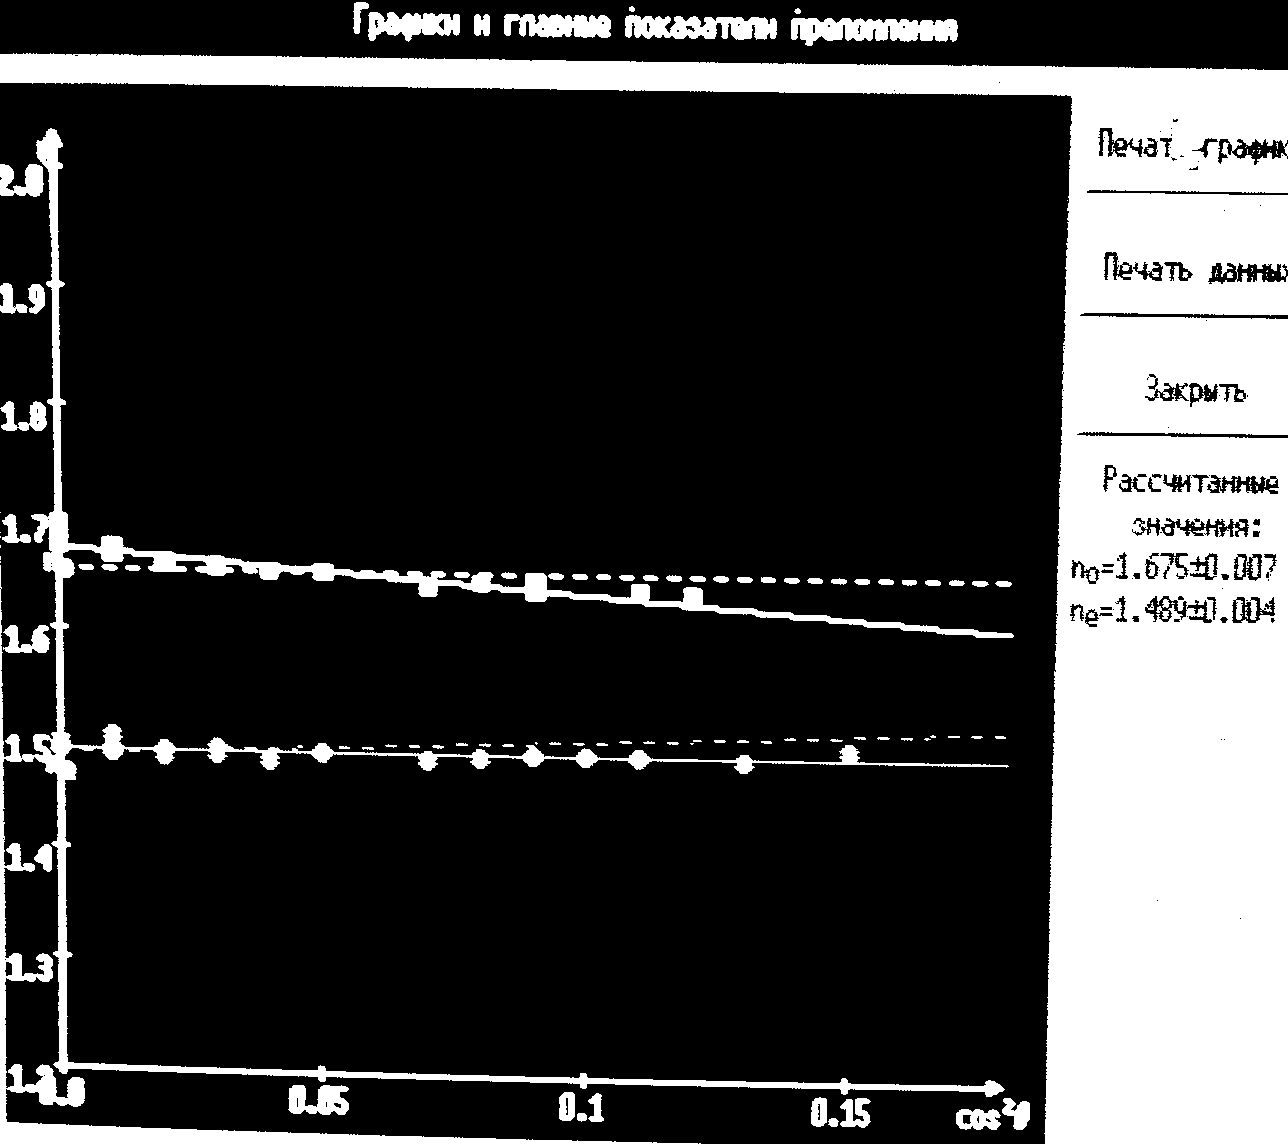
\includegraphics[width = 0.8 \textwidth]{screen.png}
	\caption{Графики и главные показатели преломления.}
\end{figure}

Из графиков получаем значения
\begin{gather*}
	n_o = 1.675 \pm 0.017, \\
	n_e = 1.489 \pm 0.013,
\end{gather*}
что хорошо согласуется с табличными данными. 

Рассчитаем средние значения углов наименьшего отклонения
\begin{gather*}
	\psi_{mo} = 26 \pm 1^{\circ}, \\
	\psi_{me} = 21 \pm 1^{\circ}.
\end{gather*}
Расчёты показателей преломления с помощью универсальной зависимости дают
\begin{gather*}
	n_o = 1.67 \pm 0.03, \\
	n_e = 1.5 \pm 0.04.
\end{gather*}

Углы падения, соответствующие полному внутреннему отражению:
\begin{gather*}
	\varphi_{1o} = 2.5 \pm {0.5}^{\circ}, \\
	\varphi_{1e} = 5.0 \pm {0.5}^{\circ}.
\end{gather*}
Через углы наименьшего отклонения определяем
\begin{gather*}
	n_o = 1.65 \pm 0.07, \\
	n_e = 1.48 \pm 0.06.
\end{gather*}

\paragraph{Вывод.}
Изучив явление двойного лучепреломления, мы измерили главные показатели преломления тремя различными способами -- и получили их взаимное согласие в пределах погрешностей.

\end{document}